\section{Evaluation}\label{sec:eval}

We measure an implementation of the \emph{Reverse Cuckoo} DMPF
(\sectionref{sec:revCuckoo}) integrated into a Ring-LPN OLE pipeline
(\sectionref{sec:ringlpn}). Waterfall's modeled costs appear separately in
\sectionref{sec:waterfallParameters}.
\sectionref{sec:RevCuckooPerf} measures the DMPF alone.
\sectionref{sec:pcgPerm} measures the end-to-end Ring-LPN OLE pipeline
and compares it with OLE and Beaver-triple baselines.

All timings predate the AES rekeying in \appendixref{app:dpf-aes}.
The OLE measurements also predate the per-expansion mask refresh in
\sectionref{sec:stationary} and omit the support-rejection filter used by
the current parameter recipe. The current implementation refreshes the
masks and filters supports at the analyzed Goldilocks point, but the tables
have not been remeasured. These results describe the
earlier revision, not validation of the complete current recipe.

\paragraph{Environment.}
Benchmarks used an i7-13700H CPU with 32\,GB DDR5 memory and local sockets
with sub-millisecond latency and bandwidth above 10\,Gbps.
All code was compiled with full optimizations (\texttt{-O3}, LTO) and native CPU tuning
(\texttt{-march=native}). Results are single-threaded per party.


\subsection{Reverse-Cuckoo DMPF}\label{sec:RevCuckooPerf}

% Requires: \usepackage{booktabs}
\begin{table}[t]
\centering
\caption{RevCuckoo DMPF time breakdown (u64 field; linear sec.\ 40; cuckoo sec.\ 2; 3 expansion calls; 1 set). Setup is measured up through \texttt{sparseDpf done} and \texttt{negate done}; time shown is the max of Party~0/1 timestamps.}
\label{tab:dmpf-time-split}
\small
\begin{tabular}{@{}llrrrr@{}}
\toprule
$n$ & $t$ & Setup [ms] & Avg.\ expand [ms] & Total [ms] & \#Expands \\
\midrule
$2^{16}$ & 16  & 72.90  & 1.37  & 77   & 3 \\
$2^{18}$ & 16  & 172.90 & 6.37  & 194  & 3 \\
$2^{20}$ & 16  & 516.20 & 27.27 & 598  & 3 \\
\midrule
$2^{16}$ & 128 & 201.80 & 2.40  & 209  & 3 \\
$2^{18}$ & 128 & 363.80 & 7.07  & 385  & 3 \\
$2^{20}$ & 128 & 988.50 & 38.50 & 1104 & 3 \\
\bottomrule
\end{tabular}

\end{table}

% Preamble:
% \usepackage{pgfplots}
% \pgfplotsset{compat=1.18}

% n = 2^18, t = 128 — Setup to negate done
% ms:  dedup 9.8, perm+hash 3.5, solve 107, sparse sets 100, sparse DPF 114, other 10
% sum = 344.3 ms
% %:   2.85,       1.02,           31.07,       29.04,         33.11,        2.91
% segment centers (in %): 1.425, 3.36, 19.405, 49.46, 80.535, 98.545
\begin{figure}[H]
  \centering
  
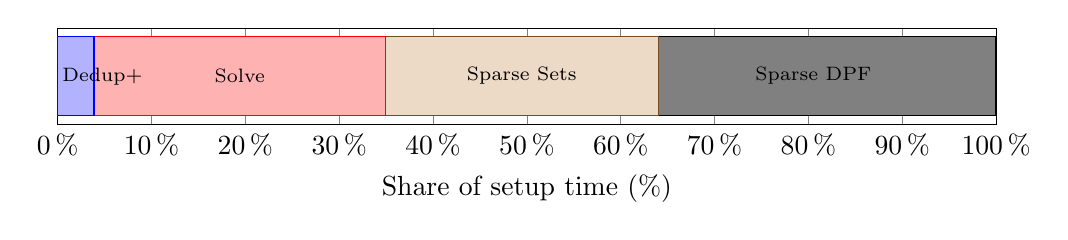
\begin{tikzpicture}
\begin{axis}[
  width=13.5cm,
  height=2.8cm,
  xbar stacked,
  xmin=0, xmax=100,
  bar width=10mm,
  ytick={1},
  yticklabels={\ },
  enlarge y limits=0.35,
  xlabel={Share of setup time (\%)},
  xtick distance=10,
  xticklabel=\pgfmathprintnumber{\tick}\,\%,
  clip=false
]

% Centered labels for each segment
\node[font=\scriptsize] at (axis cs:  4.785,1) {Dedup+ };
\node[font=\scriptsize] at (axis cs: 19.405,1) {Solve};
\node[font=\scriptsize] at (axis cs: 49.460,1) {Sparse Sets};
\node[font=\scriptsize] at (axis cs: 80.535,1) {Sparse DPF };
%\node[font=\scriptsize] at (axis cs: 98.545,1) {Other};

% Stacked segments (percent widths)
\addplot+[xbar] coordinates {( 3.87,1)};
\addplot+[xbar] coordinates {(31.07,1)};
\addplot+[xbar] coordinates {(29.04,1)};
\addplot+[xbar] coordinates {(36.00,1)};
%\addplot+[xbar] coordinates {( 2.91,1)};

\end{axis}
\end{tikzpicture}

  \caption{Reverse-Cuckoo DMPF setup breakdown at $n=2^{18},t=128$.
  Dedup+ includes deduplication, permutation, and hashing. Solve is the binary
  system solver. Sparse Sets constructs the public leaf domains; Sparse DPF
  initializes the trees and leaf values.}
  \label{fig:bar}
  
\end{figure}

\tableref{tab:dmpf-time-split} reports setup times of 72.90--988.50\,ms
and average expansion times of 1.37--38.50\,ms across the measured cases.
Expansion time increases with the domain size. Setup remains more expensive
than one expansion in every row, so reuse amortizes a substantial initial cost.



\subsection{Ring-LPN OLE pipeline}\label{sec:pcgPerm}



We generate OLE correlations over two prime fields. Goldilocks has modulus
$q=2^{64}-2^{32}+1$, whose form permits efficient modular arithmetic
\cite{goldilocks,goldilocks2}. Fp31 has modulus $q=15\cdot2^{27}+1$;
we use Montgomery reduction for this field.


\begin{table}[H]
  \centering

\begin{tabular}{|l l c | r r l l|}
\hline
Protocol & Field & $n$ & Setup time (s) & Median (op/s) & Setup comm & Expand comm \\
\hline
\hline

\SumDmpf&Goldilocks & $2^{16}$ &-- &  37,686 & --  &  12.4 MB  \\\hline
\RcDmpf&Goldilocks & $2^{16}$ & 2.628  & 885{,}621  & 149.52 MB  & 12.99 MB  \\
\RcDmpf&Goldilocks & $2^{18}$ & 3.558  & 1{,}579{,}180 & 158.92MB  & 12.99 MB  \\
\RcDmpf&Goldilocks & $2^{20}$ & 12.490 & 1{,}811{,}012 & 170.44 MB & 12.99 MB \\\hline
\cite{mp-spdz}&Goldilocks & $2^{20}$ & -- & 275,548 &-- & 176.65 MB \\\hline\hline
\SumDmpf&Fp31       & $2^{16}$ & --  & 47,250 & -- & 12.14 MB \\\hline
\RcDmpf&Fp31       & $2^{16}$ & 2.258  & 1{,}260{,}307 & 143.04 MB & 6.51 MB  \\
\RcDmpf&Fp31       & $2^{18}$ & 3.793  & 2{,}221{,}559 & 152.43 MB &  6.51 MB \\
\RcDmpf&Fp31       & $2^{20}$ & 11.583 & 2{,}709{,}498 & 163.95 MB & 6.51 MB  \\\hline
\cite{mp-spdz}&Fp31  & $2^{20}$ & -- & 309,588 & ---  & 176.56 MB  \\
\hline
\end{tabular}
\caption{Ring LPN PCG performance and communication for generating OLE correlations. For each field and vector length $n$, we report the one-time setup latency (seconds), the median per-expansion throughput over 10 expansions (op/s), and the total communication summed over both parties: one-time setup bytes and per-expansion bytes. Communication is shown in MB (decimal). \SumDmpf refers to the ``sum  of DPFs'' approach and \RcDmpf is our new Reverse Cuckoo DMPF.  \cite{mp-spdz} generates Beaver triples and therefore we generated $n'=n/2$ triples for their numbers.}
\label{tab:pcg}
  
\end{table}

The $n=2^{16}$ and $n=2^{18}$ Reverse-Cuckoo rows measure performance scaling;
they are not claimed as 40-bit correctness parameter sets for the present
degree-two feature evaluator.  \namedref{Proposition}{prop:rc-ringlpn-correctness}
and \appendixref{app:revCuckooHash} certify the corresponding filtered
$n=2^{20}$ caller distribution, not the measured unfiltered sampler.



\begin{figure}[H]
  \centering
  
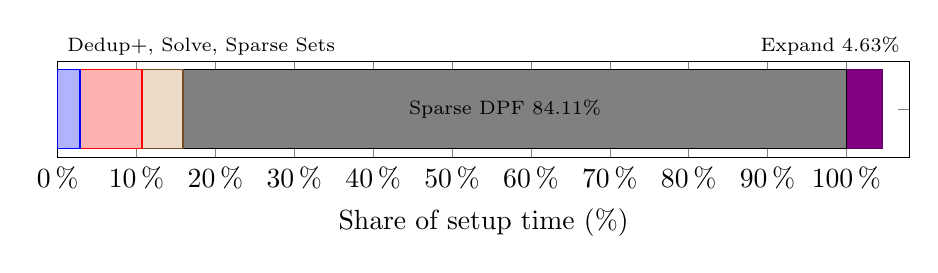
\begin{tikzpicture}
\begin{axis}[
  width=12.4cm,
  height=2.8cm,
  xbar stacked,
  xmin=0, xmax=108, % >100 to include one expansion cost
  bar width=10mm,
  ytick={1},
  yticklabels={\ },
  enlarge y limits=0.35,
  xlabel={Share of setup time (\%)},
  xtick distance=10,
  xticklabel=\pgfmathprintnumber{\tick}\,\%,
  clip=false
]

% Centered labels for each segment (positioned at segment midpoints)
\node[font=\scriptsize] at (axis cs:  1.42,1) {};
\node[font=\scriptsize,anchor=south west,yshift=16pt] at (axis cs: 0,1) {Dedup+, Solve, Sparse Sets};
\node[font=\scriptsize] at (axis cs: 13.30,1) {};
\node[font=\scriptsize] at (axis cs: 56.72,1) {Sparse DPF 84.11\%};
%\node[font=\scriptsize] at (axis cs: 98.78,1) {Other 2.44\%};
\node[font=\scriptsize,anchor=south east,yshift=16pt] at (axis cs:108,1) {Expand 4.63\%};

% Stacked segments (percent widths; first 5 sum to 100)
\addplot+[xbar] coordinates {( 2.84,1)};  % Dedup+
\addplot+[xbar] coordinates {( 7.86,1)};  % Solve
\addplot+[xbar] coordinates {( 5.19,1)};  % Sparse Sets
\addplot+[xbar] coordinates {(84.11,1)};  % Sparse DPF
%\addplot+[xbar] coordinates {( 2.44,1)};  % Other
\addplot+[xbar] coordinates {( 4.63,1)};  % 1× Expand (as % of setup)

\end{axis}
\end{tikzpicture}

  \caption{Reverse-Cuckoo Ring-LPN setup breakdown at $n=2^{20}$, with one
  expansion shown relative to setup time. Dedup+ includes deduplication,
  permutation, and hashing. Solve is the binary system solver. Sparse Sets
  constructs the public leaf domains; Sparse DPF initializes the trees and
  leaf values. The expansion measurement predates the fresh-mask update.}
  \label{fig:barPcg}
  
\end{figure}


\paragraph{Results summary.}
At $n=2^{20}$, measured throughput is 1.81 million OLEs/s in Goldilocks
and 2.71 million OLEs/s in Fp31. Relative to the measured
\cite{mp-spdz} baseline, these are throughput factors of 6.57 and 8.75.
Per-expansion communication is smaller by factors of 13.60 and 27.12.
These ratios exclude Reverse-Cuckoo setup and use the conversion of one
Beaver triple to two OLEs stated in the table caption.

At $n=2^{16}$, the throughput factors over \SumDmpf are 23.50 and 26.67.
Goldilocks expansion communication is slightly higher, not lower:
12.99\,MB versus 12.4\,MB. Fp31 uses 6.51\,MB versus 12.14\,MB.

\paragraph{Where setup time goes.}
In the $n=2^{20}$ PCG breakdown, sparse-tree initialization accounts for
84.11\% of setup time, compared with 7.86\% for solving and 5.19\% for
constructing sparse sets. The remaining 2.84\% covers deduplication,
permutation, and hashing. These are measured implementation costs, distinct
from the logical OT counts used to compare Waterfall profiles.

\paragraph{Setup amortization.}
Consider the Goldilocks row at $n=2^{20}$.
Setup takes 12.49\,s and communicates 170.44\,MB. After $Q$ expansions, total measured communication in MB is
\[
 170.44+12.99Q.
\]
For example, $Q=10$ gives 300.34\,MB.
Each expansion still communicates. The throughput column excludes setup,
so an application should account for its intended number of expansions.
We do not infer total-byte savings over the smaller-domain \SumDmpf row.

\paragraph{Field choice.}
Fp31 setup communicates 163.95\,MB at $n=2^{20}$;
Goldilocks setup communicates 170.44\,MB.
Fp31 also has higher measured throughput and a smaller expansion payload.
These differences illustrate the arithmetic tradeoff. A smaller field is
appropriate only when the application's correctness and security requirements
permit it.



